\section{Introduction}
Moving a suspect object away from people combines several robotics problems: locating a candidate, navigating toward it, positioning a gripper, transporting the object, and confirming its release. Each component can function in isolation while the complete task remains unreliable. A valid detection may arrive after its target has moved; a motion command may lose its intended magnitude at a serial gateway; an object may lie outside the arm's contact workspace even when the base has reached its navigation goal. The central engineering problem is therefore the relationship between subsystem evidence and permission to act.

Mobile robots have been developed for nuclear environments~\cite{bird2022vega}, and compact mobile manipulators demonstrate the value of integrating mobility and reach~\cite{kemp2022stretch}. HazBot addresses an accessible embedded implementation of this integration. Its central Raspberry Pi connects four functional subsystems: navigation, wheel control, visual inference, and robotic manipulation. Local perception keeps image interpretation on the robot, while dedicated embedded controllers separate sensor acquisition and actuator signaling from mission-level decisions.

We frame the application as retrieval of designated objects from a potentially hazardous area. A task specification determines which objects may be handled and where they should be deposited. Visual recognition proposes a candidate; authorization determines whether handling is permitted. This distinction accommodates task-specific detectors without treating appearance as evidence of chemical, radiological, or biological properties. Ball-based simulated control provides a nonhazardous task surrogate for the present study.

The paper makes three contributions. First, it specifies a Pi-centered four-subsystem architecture with explicit physical interfaces and separate drive, arm, and ranging controller paths. Second, it defines a seven-phase reference coordinator with observable prerequisites for mobility--manipulation handoffs. Third, it provides reproducible model and source analyses that connect these prerequisites to wrist geometry and actual command semantics. The evaluation establishes properties of the discrete coordinator and source models; physical retrieval performance remains a separate measurement problem. This scope permits precise results without borrowing detector accuracy, payload, or mission-success figures from unrelated systems.

\begin{figure*}[t]
\centering
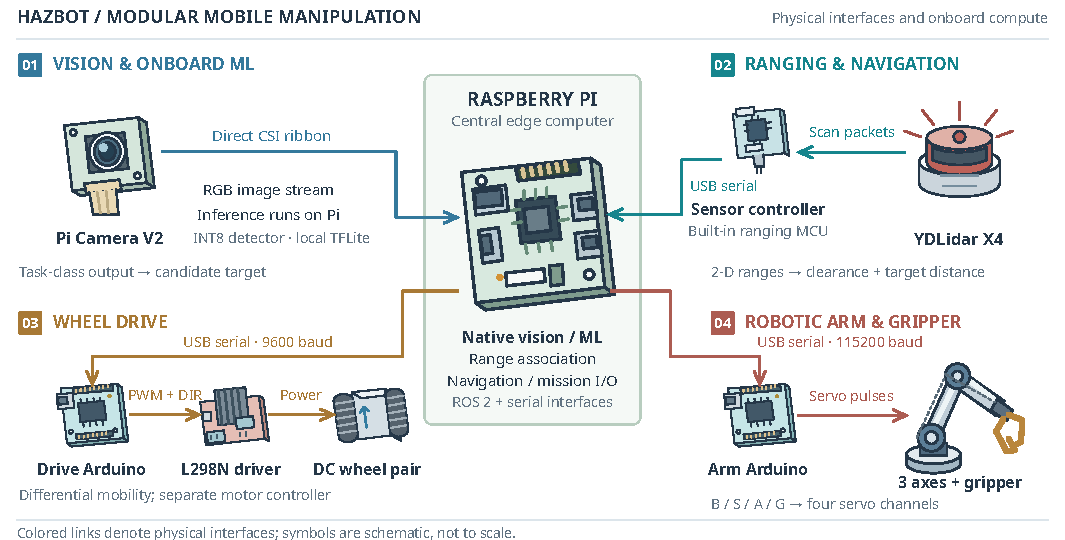
\includegraphics[width=\textwidth]{hazbot_architecture.pdf}
\caption{HazBot's four-subsystem architecture. The Raspberry Pi performs onboard computation and interfaces with a direct CSI camera, a LiDAR sensor controller, a dedicated drive Arduino, and a separate arm Arduino. Glyphs identify functional hardware; the drawing is a topology rather than a scale assembly. The complete mission coordinator is evaluated as a reference model.}
\label{fig:architecture}
\end{figure*}
